% This is samplepaper.tex, a sample chapter demonstrating the
% LLNCS macro package for Springer Computer Science proceedings;
% Version 2.20 of 2017/10/04
%
\documentclass[runningheads]{llncs}
%
\usepackage{graphicx}
\usepackage{listings}
\usepackage{xcolor}
\usepackage{multicol}
\usepackage{amsmath}

% Define settings for SPARQL code highlighting
\lstdefinelanguage{SPARQL}{
  morekeywords={PREFIX, SELECT, WHERE, FILTER, OPTIONAL, UNION},
  sensitive=true,
  morecomment=[l]{\#},
  morestring=[b][\color{blue}]\",
}
\lstset{
  language=SPARQL,
  basicstyle=\tiny\ttfamily,
  keywordstyle=\color{purple},
  commentstyle=\color{gray},
  stringstyle=\color{blue},
  showstringspaces=false,
  breaklines=true,
  tabsize=2,
}

% Used for displaying a sample figure. If possible, figure files should
% be included in EPS format.
%
% If you use the hyperref package, please uncomment the following line
% to display URLs in blue roman font according to Springer's eBook style:
% \renewcommand\UrlFont{\color{blue}\rmfamily}

\newcommand{\todo}[1]{\textit{\textcolor{magenta}{Todo: #1}}}

\begin{document}
%
\title{Near Identity Relationships}
%\title{Abstracting Entity Matching for Analysing and Explaining Identity and Difference Decision and Indecision}
%
%\titlerunning{Abbreviated paper title}
% If the paper title is too long for the running head, you can set
% an abbreviated paper title here
%
% \author{First Author\inst{1}\orcidID{0000-1111-2222-3333} \and
% Second Author\inst{2,3}\orcidID{1111-2222-3333-4444} \and
% Third Author\inst{3}\orcidID{2222--3333-4444-5555}}
% %
% \authorrunning{F. Author et al.}
% % First names are abbreviated in the running head.
% % If there are more than two authors, 'et al.' is used.
% %
% \institute{Princeton University, Princeton NJ 08544, USA \and
% Springer Heidelberg, Tiergartenstr. 17, 69121 Heidelberg, Germany
% \email{lncs@springer.com}\\
% \url{http://www.springer.com/gp/computer-science/lncs} \and
% ABC Institute, Rupert-Karls-University Heidelberg, Heidelberg, Germany\\
% \email{\{abc,lncs\}@uni-heidelberg.de}}
%
\maketitle              % typeset the header of the contribution
%
%\begin{abstract}
%The abstract should briefly summarize the contents of the paper in
%15--250 words.

%\keywords{First keyword  \and Second keyword \and Another keyword.}
%\end{abstract}
%
%
%





\subsection{Near identity relationship}
In order to evaluate if EMCs can help to identify pair of entities engaged in a near-identity relationship we provide the definition of signature and the notion of corpus.
The definition of signature is related to the definition of the most frequent context in a lattice.
\begin{definition}[Mot Frequent Context]
Given an identity (resp. difference, incompleteness) lattice, and considering the order of relations between contexts, the most frequent context is the (no empty) context which accumulates the highest number of pairs.
\end{definition}

\begin{definition}[Signature] \label{def:signature}
Given a list of EMCs, their identity, difference and incompleteness lattices, the signature is the triplet composed with the most frequent context of identity lattice, the most frequent context of difference lattice and the most frequent context of incompleteness lattice.  
\end{definition}
In the sequel we use the term \textit{corpus} and the notation $c$ to design a list of EMCs and the notation $sign$ for a signature.
It is possible to discover several signatures $S=\{sign1, sign2, ...\}$ for a given corpus. 

This discovery is done iteratively: once the first signature $sign_{1}$ has been detected on a corpus $c_{1}$, the EMCs that matched $sign1$ are removed from $c_{1}$ leading to the creation of a corpus $c_{2}$ . 
We then run a second iteration on $c_{2}$ in order to detect the next signature $sign_{2}$.
The iteration stops when a \textit{coverage} reach a given threshold. 

For a set of signatures $S$ and given initial corpus $c_{1}$, the coverage is defined by the number of EMCs that matches exactly one of the signatures in $S$ over the size of the initial corpus $c_{1}$. 
\begin{equation*}
c(S) = \frac{nb\_match\_EMCs}{size(c_{1})}
\end{equation*}



Just as key discovery is used to highlight strong identity relationships,  we would like to highlight weak identity relationships using signatures. Signatures discovery is performed on a corpus and consists in searching the most frequent contexts in this corpus. The corpus provided must be representative of a weak identity relationship: for example individuals have been linked because they refer to the same general concept such as, the book's of a writer's work or films of a director's filmography. In this use case we want to evaluate if a weak identity relationship can be described with few signatures. In other words, obtaining a coverage $c(S)$ over 80\% with a limited set of signatures $S$.


\subsubsection{Corpora construction}
We have built 5 corpora representing 2 different categories of near entity relationship. (i) relations that describe a more general concept than the one encoded in knowledge graphs (the concept of a literary or cinematographic work versus the concept of a book or film) and 
(ii) relationships that describe much more tenuous links between entities, entities linked together by their country.  
What motivated the construction of the second category was the construction of entity spaces as described by [Van Erp et \textit{al.} Toward Entity Spaces] , where the label Germany appears in three different contexts: the context of the meat industry, the context of the German population and the context of the German Davis Cup team. 
The table 1 presents for each corpus the type of entities used to build the pair, the property used to link these entities, and the number of author, director or countries present in each corpus. 
 
\begin{table}[]
    \centering
    \begin{tabular}{lcccc}
    \hline
    Corpus name & Entity 1 type & Entity 2 type & Link done on property & Nb   \\
    \hline
    &&&& \\
      \textbf{Literary Work}: books written  & & & & \\
      by the same author  & DBpedia Book & YAGO Book & author (created-inv) & 4928 authors\\
      & & & & \\
      \hline
      &&&& \\
      \textbf{Film Work}: films made  & & & & \\ 
      by the same director & DBpedia Film & YAGO Film & director (created-inv) & 8500 film directors \\
      & & & & \\
    \hline
    \hline
    &&&& \\
     \textbf{Book University}: books and & & & & \\ 
     universities located in the & & & & \\
     same country & DBpedia Book & DBpedia University & islocatedin & 126 countries \\
     & & & & \\
     \hline
     &&&& \\
     \textbf{Book Mountain}: books and &&&& \\
     mountains located in the &&&& \\
     same country& DBpedia Book & DBpedia Mountain & islocatedin & 143 countries\\
     & & & & \\
     \hline
     &&&& \\
     \textbf{Mountain University}: &&&& \\
     mountains and universities  &&&& \\
     located in the same country& DBpedia Mountain & DBedia University & islocatedin & 598 countries \\
     & & & & \\
     \hline
    \end{tabular}
    \caption{Description of the 5 corpora.}
    \label{tab:corpus-construction}
\end{table}

\subsubsection{Signature Detection}
To explicit signatures detection we present here a toy example. The table 2 presents a corpus computed from pairs of books of Agatha Christie. The pairs share the same author in each case, but titles (label) differs and the number of pages or the isbn number are missing.  
The most frequent identity context is $\{created-inv\}$, the most frequent difference context is $\{label\}$, the most frequent incompleteness context is $\{has\-pages\}$. 
The last line of the table represents the signature as the concatenation of the 3 most frequent contexts. 
Notice that in this toy example, all the EMCs matches with the first signature detected (we obtain a coverage of 100\%) we do not need a second iteration.

\subsubsection{Signature Discovery and Coverage}
In the same idea we performed signature discovery (i) on the Literary Work and Film Work corpora and (ii) on the 3 corpora of books, mountains and universities from the same country. The first row of Table 3 shows that 90\% of the pairs from the literary works corpus are recognized by a single signature $s1=\{created-inv\},\{skos:preflabel\},\{wascreatedonyear\}$. The second line shows that 2 signatures ($s2$ and $s3$) need to be combined for 90\% of the pairs in the cinematographic corpus to be recognized. The second part of Table 3 shows that 96\% of pairs from the book-mountain and book-university corpora are recognized by the same signature. 
But it takes a combination of 4 signatures to recognize 98\% pairs of the mountain-university corpus.
It appears that, on the 5 corpora studied, it is possible to summarize near-identity relationships with few singatures. 

\begin{table}[]
    \centering
    \begin{tabular}{llll}
        \multicolumn{4}{l}{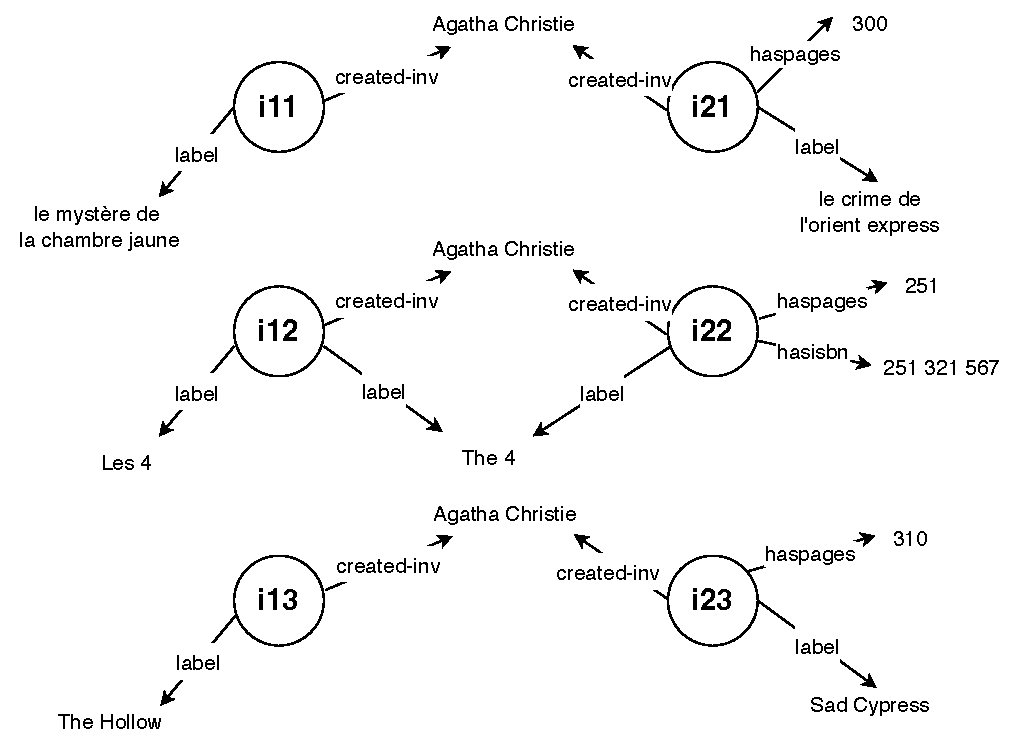
\includegraphics[scale=0.7]{./agatha.pdf}} \\
        %\hline
         i11,i21 & \{created-inv\}& \{label\}&\{haspages\} \\
         i12,i22 & \{created-inv,label\}&\{label\} &\{haspages,hasisbn\} \\
         i13,i23 & \{created-inv\}&\{label\}&\{has-pages\}\\
        \hline
        
        signature & \{created-inv\}&\{label\}&\{has-pages\} \\
        
    \end{tabular}
    \caption{The example of signature construction based on 3 EMCs.}
    \label{tab:signature_example}
\end{table}

\begin{table}[]
    \centering
    \begin{tabular}{l|l|c|c|c}
        \hline
         corpus & signature $\varepsilon\Delta\Omega$ & nb match & total nb EMCs & coverage   \\
         \hline
       literary work  & & & & \\
         & s1=\{created-inv\},\{skos:preflabel\},\{wascreatedonyear\}& & & \\
       \hline  
       & s1 & 148281 & 165508 & 0.90\\
       \hline
       film work & & & & \\  
       & s2=\{directed-inv\}\{skos:preflabel\},\{wascreatedonyear\} & & & \\
       & s3=\{directed-inv\}\{skos:preflabel\},\{islocatedin\} & & & \\
       \hline
        & s2 $\cup$ s3 & 606529 & 674952 & 0.90\\
       %\hline
       \hline
       \hline
       book mountain & & & & \\  
       & s4=\{islocatedin\},\{skos:preflabel\}, \{created-inv\}& & & \\
       \hline
       & s4 & 15320925 & 15993180 & 0.96\\
       \hline
       book university & & & &  \\
       & s5=\{islocatedin\},\{skos:preflabel\},\{created-inv\}& & & \\
       \hline
       & s5 & 15320840 & 15993082 & 0.96 \\
       \hline
       mountain university  & & & & \\
       & s6=\{islocatedin\},\{islocatedin\},\{haslatitude\}, \{haslongitude\}& & & \\
       &s7=\{islocatedin\},\{islocatedin\},\{graduatedfrom-inv\}& & & \\
       &s8=\{islocatedin\}\{islocatedin\},\{\}& & & \\
       &s9=\{islocatedin\}\{islocatedin\},\{hasmotto\}& & & \\
       \hline
       &s6 $\cup$ s7 $\cup$ s8 $\cup$ s9 & 4708646 & 4795678& 0.98\\
       \hline
    \end{tabular}
    \caption{signatures detection on corpora}
    \label{tab:signature_detection}
\end{table}

\subsection{Code}
Corpora construction, signature detection and coverage computation are available in the following scripts:
\begin{itemize}
	\item iswc2024/pattern/author\_work\_pattern.py for the corpus author work
	\item iswc2024/pattern/director\_work\_pattern.py for the corpus cinematographic work
	\item iswc2024/pattern/country\_work\_pattern.py for the 3 corpora of entities linked by their countries 
\end{itemize}

\end{document}
